\documentclass[border=6pt]{standalone}
\usepackage[utf8]{inputenc}
\usepackage[T1]{fontenc}
\usepackage{lmodern}
\usepackage{tikz}
\usetikzlibrary{shapes.geometric, arrows.meta, positioning, calc}

\begin{document}
\sffamily
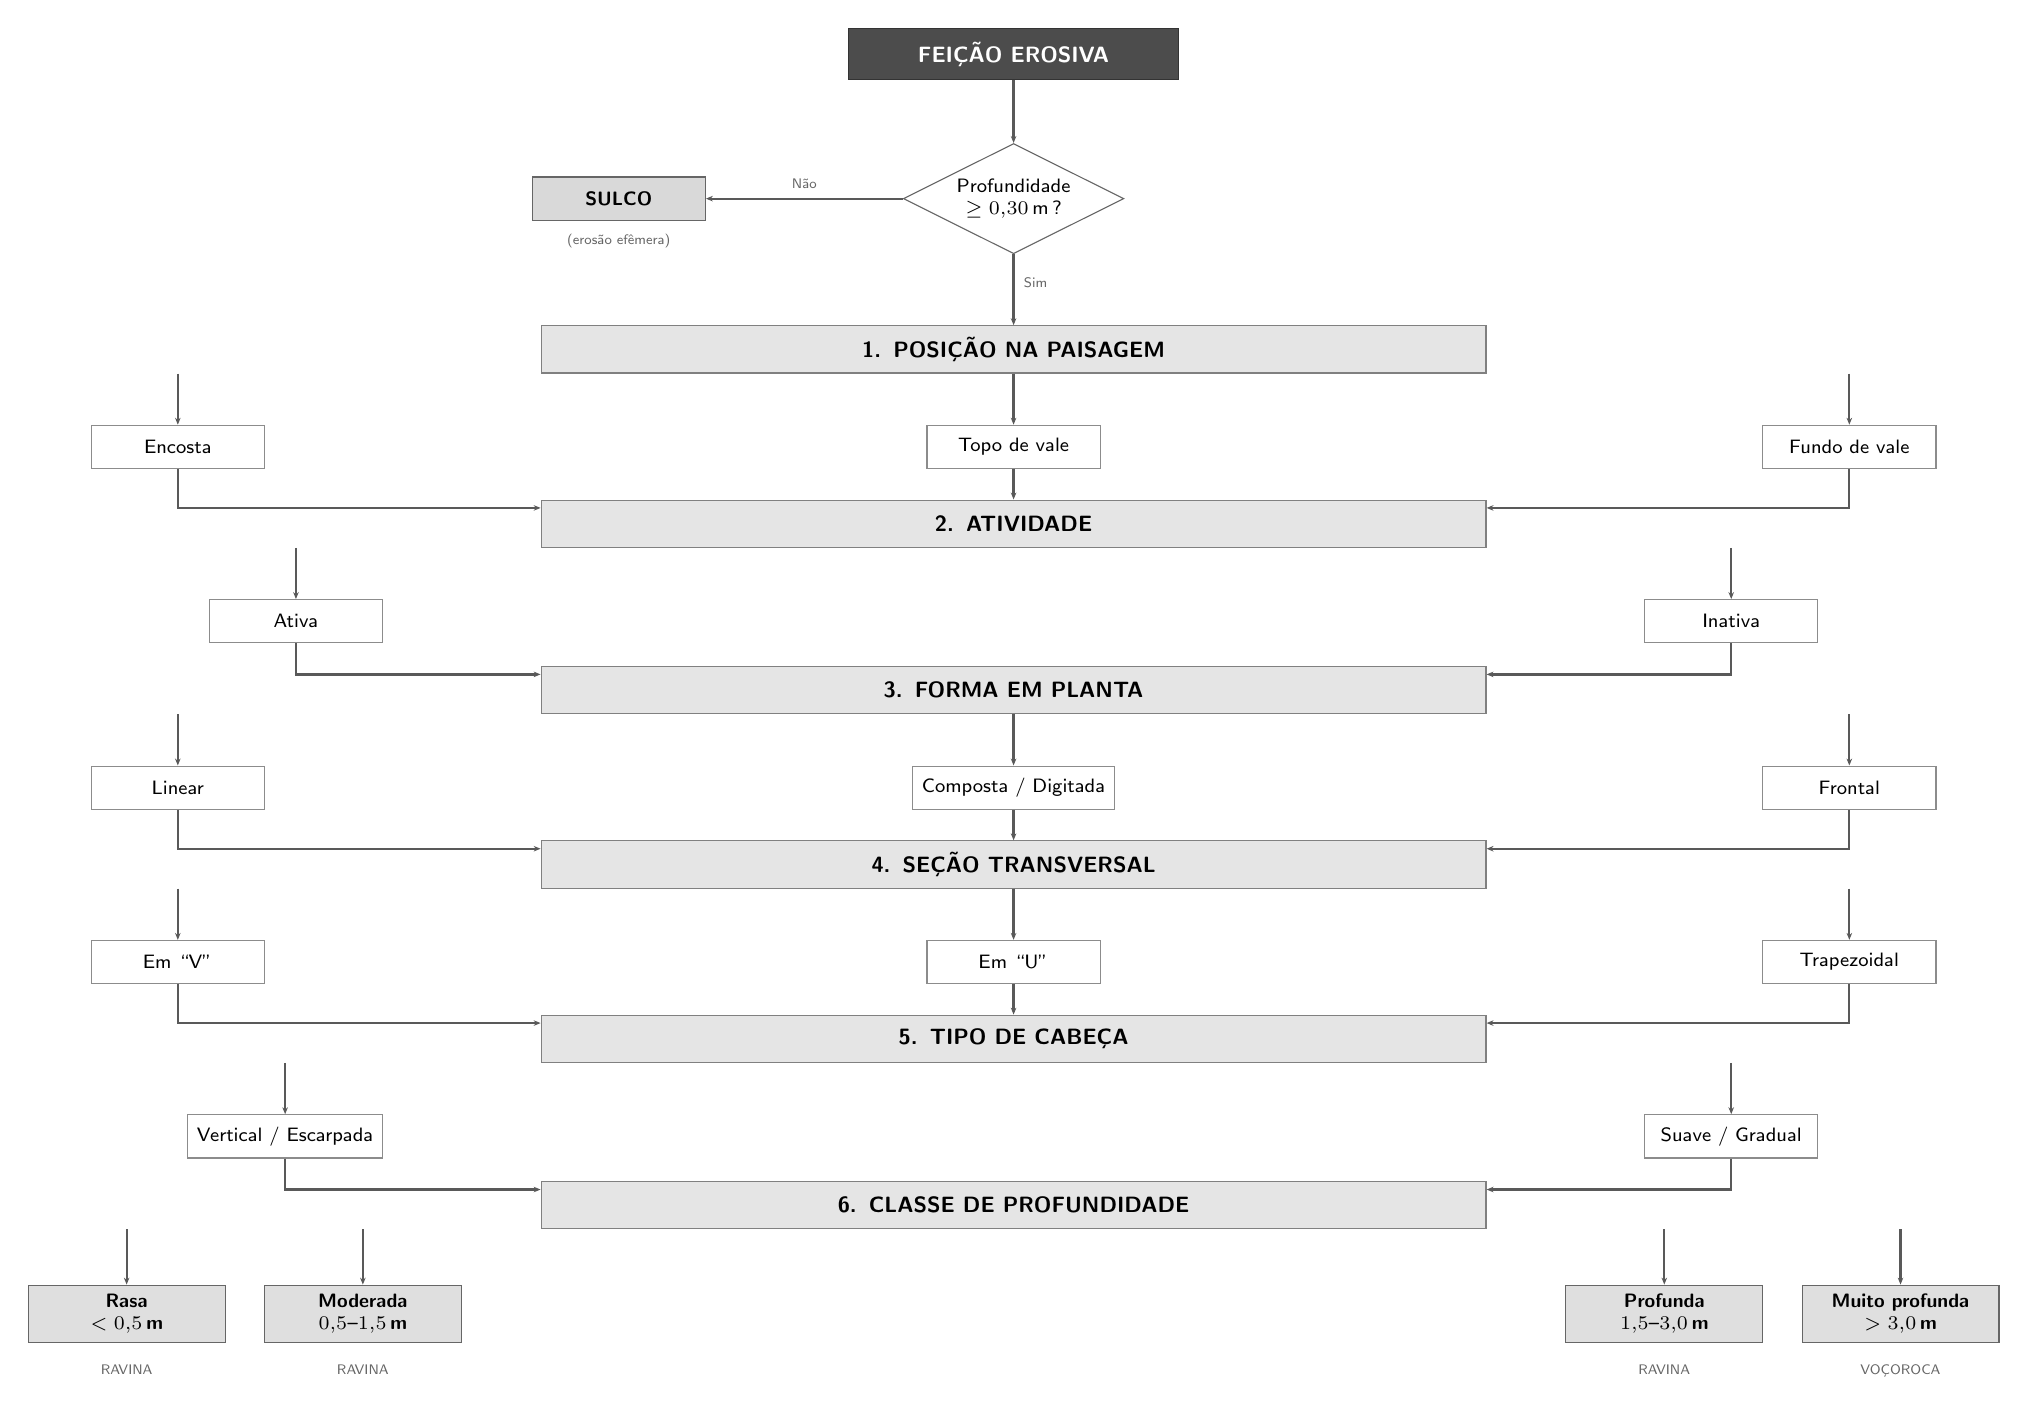
\begin{tikzpicture}[
    node distance=0.9cm and 0.3cm,
    every node/.style={font=\sffamily\footnotesize},
    % Header style (dark)
    header/.style={
        rectangle, draw=black!80, fill=black!70, text=white,
        minimum width=4.2cm, minimum height=0.65cm, align=center,
        font=\sffamily\footnotesize\bfseries
    },
    % Criteria bar (medium gray)
    criteria/.style={
        rectangle, draw=black!50, fill=gray!20,
        minimum width=12cm, minimum height=0.6cm, align=center,
        font=\sffamily\footnotesize\bfseries
    },
    % Decision diamond
    decision/.style={
        diamond, draw=black!60, fill=white,
        minimum width=2.8cm, minimum height=1.4cm, align=center,
        inner sep=1pt, font=\sffamily\scriptsize, aspect=2.2
    },
    % Option box (white)
    option/.style={
        rectangle, draw=black!45, fill=white,
        minimum width=2.2cm, minimum height=0.55cm, align=center,
        font=\sffamily\scriptsize
    },
    % Terminal classification box
    terminal/.style={
        rectangle, draw=black!60, fill=gray!25,
        minimum width=2.5cm, minimum height=0.55cm, align=center,
        font=\sffamily\scriptsize\bfseries
    },
    % Exit/end box (darker)
    exitbox/.style={
        rectangle, draw=black!60, fill=black!15,
        minimum width=2.2cm, minimum height=0.55cm, align=center,
        font=\sffamily\scriptsize\bfseries
    },
    % Arrow style
    arr/.style={-{Stealth[length=2.5pt, width=2pt]}, black!65, thick},
    % Label style
    lbl/.style={font=\sffamily\tiny, black!60}
]

% ===== LEVEL 0: Entry =====
\node (entry) [header] {FEI\c{C}\~{A}O EROSIVA};

% ===== LEVEL 1: Depth decision =====
\node (depth) [decision, below=0.8cm of entry] {Profundidade\\$\geq 0{,}30\,$m\,?};
\draw [arr] (entry) -- (depth);

% Sulco exit (left)
\node (sulco) [exitbox, left=2.5cm of depth] {SULCO};
\draw [arr] (depth) -- node[lbl, above] {N\~{a}o} (sulco);
\node [lbl, below=0.05cm of sulco] {(eros\~{a}o ef\^{e}mera)};

% ===== LEVEL 2: Landscape position =====
\node (pos_bar) [criteria, below=0.9cm of depth] {1.\enspace POSI\c{C}\~{A}O NA PAISAGEM};
\draw [arr] (depth) -- node[lbl, right, pos=0.4] {Sim} (pos_bar);

\node (enc)   [option, below left=0.65cm and 3.5cm of pos_bar]  {Encosta};
\node (topo)  [option, below=0.65cm of pos_bar]                 {Topo de vale};
\node (fundo) [option, below right=0.65cm and 3.5cm of pos_bar] {Fundo de vale};
\draw [arr] (pos_bar.south -| enc)  -- (enc);
\draw [arr] (pos_bar.south)         -- (topo);
\draw [arr] (pos_bar.south -| fundo) -- (fundo);

% ===== LEVEL 3: Activity =====
\node (ativ_bar) [criteria, below=1.6cm of pos_bar] {2.\enspace ATIVIDADE};
\draw [arr] (enc.south)   |- ([yshift=0.2cm]ativ_bar.west);
\draw [arr] (topo.south)  -- (ativ_bar);
\draw [arr] (fundo.south) |- ([yshift=0.2cm]ativ_bar.east);

\node (ativa)   [option, below left=0.65cm and 2cm of ativ_bar]  {Ativa};
\node (inativa) [option, below right=0.65cm and 2cm of ativ_bar] {Inativa};
\draw [arr] (ativ_bar.south -| ativa)  -- (ativa);
\draw [arr] (ativ_bar.south -| inativa) -- (inativa);

% ===== LEVEL 4: Plan form =====
\node (forma_bar) [criteria, below=1.5cm of ativ_bar] {3.\enspace FORMA EM PLANTA};
\draw [arr] (ativa.south)   |- ([yshift=0.2cm]forma_bar.west);
\draw [arr] (inativa.south) |- ([yshift=0.2cm]forma_bar.east);

\node (linear)   [option, below left=0.65cm and 3.5cm of forma_bar]  {Linear};
\node (digitada) [option, below=0.65cm of forma_bar]                  {Composta / Digitada};
\node (frontal)  [option, below right=0.65cm and 3.5cm of forma_bar] {Frontal};
\draw [arr] (forma_bar.south -| linear)   -- (linear);
\draw [arr] (forma_bar.south)             -- (digitada);
\draw [arr] (forma_bar.south -| frontal)  -- (frontal);

% ===== LEVEL 5: Cross-section =====
\node (secao_bar) [criteria, below=1.6cm of forma_bar] {4.\enspace SE\c{C}\~{A}O TRANSVERSAL};
\draw [arr] (linear.south)   |- ([yshift=0.2cm]secao_bar.west);
\draw [arr] (digitada.south) -- (secao_bar);
\draw [arr] (frontal.south)  |- ([yshift=0.2cm]secao_bar.east);

\node (vshape) [option, below left=0.65cm and 3.5cm of secao_bar]  {Em ``V''};
\node (ushape) [option, below=0.65cm of secao_bar]                  {Em ``U''};
\node (trap)   [option, below right=0.65cm and 3.5cm of secao_bar] {Trapezoidal};
\draw [arr] (secao_bar.south -| vshape) -- (vshape);
\draw [arr] (secao_bar.south)           -- (ushape);
\draw [arr] (secao_bar.south -| trap)   -- (trap);

% ===== LEVEL 6: Head type =====
\node (cab_bar) [criteria, below=1.6cm of secao_bar] {5.\enspace TIPO DE CABE\c{C}A};
\draw [arr] (vshape.south) |- ([yshift=0.2cm]cab_bar.west);
\draw [arr] (ushape.south) -- (cab_bar);
\draw [arr] (trap.south)   |- ([yshift=0.2cm]cab_bar.east);

\node (vert)  [option, below left=0.65cm and 2cm of cab_bar]  {Vertical / Escarpada};
\node (suave) [option, below right=0.65cm and 2cm of cab_bar] {Suave / Gradual};
\draw [arr] (cab_bar.south -| vert)  -- (vert);
\draw [arr] (cab_bar.south -| suave) -- (suave);

% ===== LEVEL 7: Depth class (terminal) =====
\node (prof_bar) [criteria, below=1.5cm of cab_bar] {6.\enspace CLASSE DE PROFUNDIDADE};
\draw [arr] (vert.south)  |- ([yshift=0.2cm]prof_bar.west);
\draw [arr] (suave.south) |- ([yshift=0.2cm]prof_bar.east);

\node (rasa)  [terminal, below left=0.7cm and 4cm of prof_bar]  {Rasa\\$< 0{,}5\,$m};
\node (mod)   [terminal, below left=0.7cm and 1cm of prof_bar]  {Moderada\\$0{,}5$--$1{,}5\,$m};
\node (prof)  [terminal, below right=0.7cm and 1cm of prof_bar] {Profunda\\$1{,}5$--$3{,}0\,$m};
\node (mprof) [terminal, below right=0.7cm and 4cm of prof_bar] {Muito profunda\\$> 3{,}0\,$m};
\draw [arr] (prof_bar.south -| rasa)  -- (rasa);
\draw [arr] (prof_bar.south -| mod)   -- (mod);
\draw [arr] (prof_bar.south -| prof)  -- (prof);
\draw [arr] (prof_bar.south -| mprof) -- (mprof);

% ===== TERMINAL LABELS =====
\node [lbl, below=0.15cm of rasa]  {RAVINA};
\node [lbl, below=0.15cm of mod]   {RAVINA};
\node [lbl, below=0.15cm of prof]  {RAVINA};
\node [lbl, below=0.15cm of mprof] {VO\c{C}OROCA};

\end{tikzpicture}
\end{document}
